\chapterimage{images/persistency/persistence.jpg}

\chapter{Persistence}
In this Chapter we will review some of the persistence methods use in Android. We will have a look into saving a small portion of data and a more structured (relational) type of data.

\section{Shared preferences}
If you have a relatively small collection of key-values that you'd like to save, you should use the SharedPreferences APIs. A SharedPreferences object points to a file containing key-value pairs and provides simple methods to read and write them. Each SharedPreferences file is managed by the framework and can be private or shared.

\subsection{Creating shared preferences}
Using the SharedPreferences class, you can create named maps of name/value pairs that can be persisted across sessions and shared among application components running within the same application sandbox. To create or modify a Shared Preference, call getSharedPreferences on the current Context, passing in the name of the Shared Preference to change.

Shared Preferences are stored within the application’s sandbox, so they can be shared between an application’s components but aren’t available to other applications. To modify a Shared Preference, use the SharedPreferences.Editor class. Get the Editor object by calling edit on the Shared Preferences object you want to change.

To save edits, call apply on the Editor object to save the changes asynchronously.
\begin{android}
SharedPreferences mySharedPreferences = getSharedPreferences(MY_PREFS, 
Activity.MODE_PRIVATE);
SharedPreferences.Editor editor = mySharedPreferences.edit();
// Store new primitive types in the shared preferences object.
editor.putBoolean("isTrue", true);
editor.putFloat("lastFloat", 1f);
editor.putInt("wholeNumber", 2);
editor.putLong("aNumber", 3l);
editor.putString("textEntryValue", "Not Empty");
editor.apply();
\end{android}


\subsection{Retrieving shared preferences}
Accessing Shared Preferences, like editing and saving them, is done using the getSharedPreferences method. Use the type-safe get methods to extract saved values. Each getter takes a key and a default value (used when no value has yet been saved for that key.)

\begin{android}
// Retrieve the saved values.
boolean isTrue = mySharedPreferences.getBoolean("isTrue", false);
float lastFloat = mySharedPreferences.getFloat("lastFloat", 0f);
int wholeNumber = mySharedPreferences.getInt("wholeNumber", 1);
long aNumber = mySharedPreferences.getLong("aNumber", 0);
String stringPreference =
mySharedPreferences.getString("textEntryValue", "");
\end{android}

\section{Room}
Android provides a built-in SQLite database for when the data you want to store is more complex than just key-value pairs.
Oftentimes this is used to provide caching and/or offline functionality: once a network request has been made the result is also saved in the applications database so it can be accessed when no network is available.

Room, just like ViewModel and LiveData, is one of the recently released Architecture Components.
It's a wrapper around the built-in SQLite functionalities.
Working directly with the SQLite API is possible, but it is very low-level and requires a great deal of time and effort to use: \cite{Sqlite}
\begin{enumerate}
	\item There is no compile-time verification of raw SQL queries.
	As your data graph changes, you need to update the affected SQL queries manually.
	This process can be time consuming and error prone.
	\item You need to use lots of boilerplate code to convert between SQL queries and data objects.
\end{enumerate}

\subsection{In theory}
There are 3 major components in Room \cite{RoomDevAndroid} (see also figure \ref{fig:roomarchitecture}):
\begin{description}
	\item[Database]: Contains the database holder and serves as the main access point for the underlying connection to your app's persisted, relational data.
	The class that's annotated with @Database should satisfy the following conditions:
	\begin{enumerate}
		\item Be an abstract class that extends RoomDatabase.
		Include the list of entities associated with the database within the annotation.
		\item Contain an abstract method that has 0 arguments and returns the class that is annotated with @Dao.
	\end{enumerate}
 	At runtime, you can acquire an instance of Database by calling Room.databaseBuilder() or Room.inMemoryDatabaseBuilder().
	\item [DAO]: Contains the methods used for accessing the database.
	\item [Entity]: Represents a table within the database.
\end{description}

\begin{figure}
	\centering
	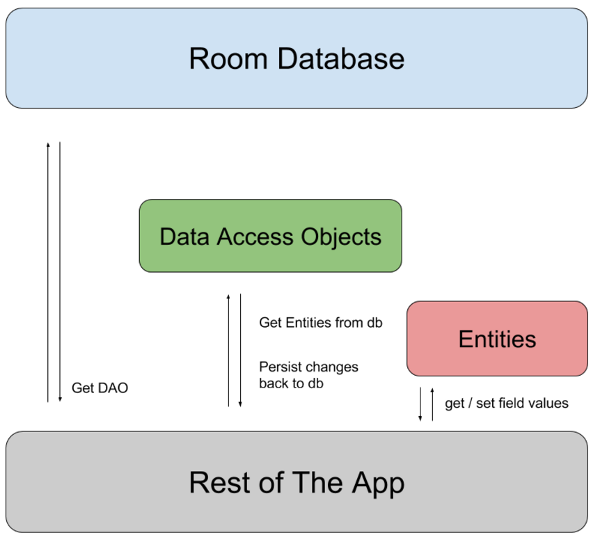
\includegraphics[width=0.7\linewidth]{images/persistency/room_architecture}
	\caption{Room architecture diagram. From \cite{RoomDevAndroid}.}
	\label{fig:roomarchitecture}
\end{figure}

\subsection{In practice}
In this section we'll follow a slightly adapter version of Google's Room with a View Codelab \cite{RoomWithAView}.
We won't be using Kotlin's co-routine feature and will also uses multiple fragments instead of multiple activities. 


\subsection{Setting up the gradle files}
After starting a new project with just an empty Activity, make the following changes to the app's build.gradle file.

Add the Kotlin annotation processor.
This processor will read the annotations we put with the Database, Entity and DAO classes.
\begin{android}
	apply plugin: 'kotlin-kapt'
\end{android}

And add the necessary libraries:
\begin{android}
// Room components
implementation "android.arch.persistence.room:runtime:1.1.1"
kapt "android.arch.persistence.room:compiler:1.1.1"
androidTestImplementation "android.arch.persistence.room:testing:1.1.1"

// Lifecycle components
implementation "android.arch.lifecycle:extensions:1.1.1"
kapt "android.arch.lifecycle:compiler:1.1.1"
\end{android}

\subsection{Creating the entity}
Every class you want to save in the database has to become a database \textit{entity}.
In this simple application we will allow the user to add words to a database.

This means creating a Word class and giving it the required annotations.
\begin{description}
	\item[@Entity] is used to indicate to the Room library that objects of this class will be stored in the database.
	The annotation also requires a tableName parameter that specifies the name of the table in which the objects will be stored.
	\item[@PrimaryKey] indicates, as you would expect, which attribute is the primary key for this table.
	\item[@ColumnInfo] can be used if you want the column name to be different from the name of the attribute.
\end{description}

\begin{android}
@Entity(tableName = "word_table")
class Word(@PrimaryKey @ColumnInfo(name = "word") val word: String)
\end{android}

\subsection{Creating the DAO}
A DAO is a \textbf{D}ata \textbf{A}ccess \textbf{O}bject.
With this object Room allows us to write the required SQL queries. 
Just like in Retrofit we define an interface (an abstract class is possible as well) with the methods we'd like to call and annotate each method with the corresponding SQL query.

Room provides some predefined annotations for the most common queries (@Insert, @Update, @Delete).
For other queries the @Query annotation should be used, with the actual query as parameter for the annotation.

\begin{android}
/**
* Use the @Query annotation to specify a custom SQL query.
* By specifiying LiveData as the return value Room will provide all the necessary code to update the LiveData object
* when the database is updated.
*/
@Query("SELECT * from word_table ORDER BY word ASC")
fun getAllWords(): LiveData<List<Word>>


@Insert
fun insert(word: Word)

@Query("DELETE FROM word_table")
fun deleteAll()
\end{android}

\subsection{Adding a database}
The DAO itself isn't enough to perform the queries.
Just like a Retrofit API needs a backend to respond to the requests, we need a database to query. 

The database class should be abstract and extend RoomDatabase.
The @Database annotation is used to indicate what entities the database will hold, as well as indicate a version number
\footnote{This version number can be upped each time you make changes to the database scheme. 
	If you want to migrate the data from one schema version to the next you'll have to write Migration classes and include them when building the database.
	More info on \url{https://medium.com/androiddevelopers/understanding-migrations-with-room-f01e04b07929}.}
Every DAO that will be used to perform queries on this database should be mentioned as return values for abstract functions.
When building the database these interfaces will be implemented for you.

The database class should also be implemented as a singleton to avoid multiple instances of your database being opened at the same time.

\begin{android}
@Database(entities = [Word::class], version = 1)
abstract class WordDatabase : RoomDatabase() {
	abstract fun wordDao(): WordDao
	
	companion object {
		@Volatile
		private var INSTANCE: WordDatabase? = null
		
		fun getDatabase(context: Context): WordDatabase {
			val tempInstance = INSTANCE
			if (tempInstance != null) {
				return tempInstance
			}
			synchronized(this) {
				val instance = Room.databaseBuilder(
					context.applicationContext,
					WordDatabase::class.java,
					"Word_database"
				).build()
				INSTANCE = instance
				return instance
			}
		}
	}
}
\end{android}

\subsection{The repository pattern}
You've known about repositories since your first year: they're classes that represent a collection of objects and the ones that are responsible for communication with the persistence layer of you application. 
This latter is what we'll be doing here: the repository class will abstract the access to multiple data sources (network and database).
A simple diagram is shown in figure \ref{fig:repository}.

\begin{figure}
	\centering
	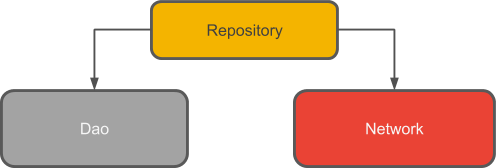
\includegraphics[width=0.7\linewidth]{images/persistency/repository}
	\caption{A Repository class abstracts access to multiple data sources.
		When a network connection is unavailable, the Dao can be used to request cached data instead.
		Using the repository pattern hides this complexity from other classes.}
	\label{fig:repository}
\end{figure}

The repository usually implements the logic for deciding whether to fetch data from a network or use results cached in a local database.
In this simple example we'll only implement the database portion. 

For every operation a method should be implemented. 
These methods will call the corresponding DAO.
Database calls should always be done asynchronously to avoid blocking the main thread.
To enforce this we add the @WorkerThread annotation to each method.

\begin{android}
class WordRepository(private val wordDao: WordDao) {
	val words: LiveData<List<Word>> = wordDao.getAllWords()
	
	@WorkerThread
	fun insert(word: Word) {
		wordDao.insert(word)
	}
}
\end{android}


\subsection{Using the DAO}
We will use a ViewModel to hold the list of all words that have been entered.
This ViewModel will have to load the list from the database when it is created, and provide a function that inserts a given word into the database.
To do this it needs a WordRepository.

\begin{android}
class WordViewModel : ViewModel() {
	@Inject
	lateinit var wordRepository: WordRepository
	
	init {
		App.component.inject(this)
	}
	
	val allWords: LiveData<List<Word>> = wordRepository.words
	
	fun insert(word: Word) {
		doAsync {
			wordRepository.insert(word)
		}
	}
}
\end{android}

The wordRepository is injected using Dagger. 
How this is done is slightly different from the way explained in the network chapter:
to create a SQLite database you require a context. 
You can't create a context object yourself, so it has to be given to the Module somehow. 
This is done by creating our own Application class, registering it in the manifest file, and passing itself as a constructor parameter for the Module.
The created component is saved in a companion object and can thus be used everywhere throughout our app.

\begin{android}	
class App : Application() {
	companion object {
		lateinit var component: DatabaseComponent
	}
	
	override fun onCreate() {
		super.onCreate()
		component = DaggerDatabaseComponent
						.builder()
						.databaseModule(DatabaseModule(this))
						.build()
	}
}
\end{android}

This ViewModel is now ready to be used.
In a MainFragment we create the ViewModel and ask it for the list of words so we can fill the RecyclerView.
In a NewWordFragment we allow the user to enter a word and ask the ViewModel to save it (to the database).

\subsection{Persisting relations}
Room does not allow Entities inside other Entities\cite{RoomDevTalk}.
This might seem like a burden, but there's a good reason. 
When querying for an Entity that has a relationship with an other Entity, you do not always want the related object as well.
Some ORM-tools solve this by implementing lazy loading: the related Entity is only queried when specifically asked for.
This can cause problems when, for example, implementing a RecyclerView with many instances of the first Entity.
If each ViewHolder would also ask for the related Entity, suddenly you're making lots of queries at once, and possibly slowing down your app.
For this reason, the Room developers disallowed this kind of behavior.

That of course doesn't mean that you can't use relations at all in Room.
You can just only use them in ways that avoid nasty scenario's like the one described above. 

There are two options (that can be combined as well):
\begin{enumerate}
	\item Don't keep a reference (relation) to other Entities.
		Instead, link them purely by using ID's and manually query for the relation when you need it.
		The @ForeignKey annotation provided by Room can help you keep the relations up-to-date by specifying what happens when one side of the relationship is deleted or updated.
	\item Explicitly ask for the relation when querying an Entity. 
		This is done using the @Relation annotation.		
\end{enumerate}

Both options are implemented in a small sample app found on \url{https://github.com/hdeweirdt/TVShows}.
It allows the user to add Shows to a list and click on one of the Shows and add Episodes for it.
The RecyclerViews displaying the Shows and Episodes are automatically updated when a new item is added.

The \textit{foreign\_keys} branch implements the first option.
The \textit{relations} branch continues on the first but uses the @Relation annotation to request both a Show and its Episodes at the same time.

\subsubsection{Foreign Keys}
When using only the Foreign Keys annotation there's no need for a Show to remember a list of its Episodes.
When we need the Episodes, we can query for them by using the Show's ID.

Let's first look at the code for the Show:
\begin{android}
@Entity(tableName = "show_table", indices = [(Index(value = ["id"], unique = true))])
@Parcelize
data class Show(
	val title: String,
	@PrimaryKey
	val id: UUID = UUID.randomUUID()) : Parcelable
\end{android}
We still use the Entity annotation, but now also add an ``indices'' parameter. 
This instructs SQLite to create an index on the specified column.
This is optional but speeds up SELECT WHERE queries (and slows down writes and updates).

The code for an Episode illustrates the ForeignKey annotation:
\begin{android}	
@Entity(tableName = "episode_table",
		indices = [(Index(value = ["id"], unique = true)), (Index(value = ["showID"], unique = false))],
		foreignKeys = [ForeignKey(
			entity = Show::class,
			parentColumns = ["id"],
			childColumns = ["showID"],
			onDelete = ForeignKey.CASCADE,
			onUpdate = ForeignKey.CASCADE)])
data class Episode(
	val title: String,
	val showID: UUID,
	@PrimaryKey
	val id: UUID = UUID.randomUUID())
\end{android}

Here we again define the tableName and the indices.
The foreignKey is an extra attribute for the Entity annotation.
In it we describe PK-FK relationship between Show and Episodes.
In parentColumn we refer to the id attribute in Show, as it is the PK. 
The childColumn is the FK: here it is the showID from Episode. 

With the onDelete and onUpdate you can specify what happens when a Show is deleted or updated.
Options are CASCADE (also delete or update), RESTRICT (don't allow, so throw an error), NO\_ACTION (self-explanatory) and SET\_NULL(same).

We'll have two separate DAO's: one for Shows and one for Episodes.
Putting all queries together in a single DAO is possible but with a rising number of queries the interface would soon become an unstructured mess.
The ShowDao will be used most. The code can be found below:
\begin{android}
@Query("SELECT * from show_table")
fun getAllShows(): LiveData<List<Show>>

@Insert(onConflict = OnConflictStrategy.REPLACE)
fun insert(show: Show)

@Query("SELECT * FROM show_table WHERE id=:showId")
fun getShow(showId: UUID): LiveData<Show>

@Query("SELECT * FROM episode_table WHERE showID=:showId")
fun getEpisodesFromShow(showId: UUID): LiveData<List<Episode>>

@Query("DELETE FROM show_table WHERE id=:showId")
fun deleteShow(showId: UUID)

@Query("DELETE FROM show_table")
fun deleteAll()	
\end{android}

In getEpisodesFromShow we query for the Episodes belonging to a specific Show.
When using just Foreign Keys there's no way to automatically receive a Show object together with all its Episodes.
This might be good or bad, depending on what you need or want.
Using relations, as described in the next section, does allow this.

\subsubsection{Relations}
The previous subsection illustrated using Foreign Keys.
Their main advantage is that you can define what happens when the parent Entity in the relation is deleted or updated.
The downside is that Shows and Episodes exist separately.

Room allows querying both parts of a relationship automatically by using the @Relation annotation.
This has to be used in a POJO\footnote{Plain Old Java Object}.

See the following code:
\begin{android}
class ShowWithEpisodes(
	@Embedded
	var show: Show? = null,
	@Relation(parentColumn = "id", entityColumn = "showId", entity = Episode::class)
	var episodes: List<Episode> = mutableListOf())
\end{android}

The @Embedded annotation will allow SQlite to reference the fields in Show directly.
This means that when Room can fill in the results of a query with fields from Show directly into a Show object.
The @Relation defines the relation that will be fetched.
Using the id field from Show (which can be referenced because we used the @Embedded annotation) and the showId from the Episodes Room can find out which Episodes belong to the Show and use them to fill in the episodes list.

The DAO changes slightly: we no longer receive Shows and Episodes, but objects of the ShowWithEpisodes class:
\begin{android}
@Transaction
@Query("SELECT * FROM show_table")
fun getAllShowsWithEpisodes() : LiveData<List<ShowWithEpisodes>>

@Transaction
@Query("SELECT * FROM show_table where id= :showId")
fun getSingleShowWithEpisodes(showId: UUID) : LiveData<ShowWithEpisodes>
\end{android}
We use the @Transaction annotation to make sure both queries (the one for the Show and the one for the Show's Episodes) are run together.

Now, we don't want to work with objects of ShowWithEpisode, but with Shows that have their episodes list filled with the corresponding episodes.
It would be great if there was a way to map objects of ShowWithEpisode directly to Shows. 
Luckily, this is possible, and the ShowRepository is a great place to do this:
\begin{android}
fun getAllShows(): LiveData<List<Show>> {
	val showsWithEpisodes = showDao.getAllShowsWithEpisodes()
	return Transformations.map(showsWithEpisodes) {combineListOfShows(it)}
}

fun getShow(showId : UUID): LiveData<Show> {
	val showWithEpisodes = showDao.getSingleShowWithEpisodes(showId)
	return Transformations.map(showWithEpisodes) {combineSingleShow(it)}
}

private fun combineListOfShows(showsWithEpisodes: List<ShowWithEpisodes>) : List<Show> {
	return showsWithEpisodes.map{combineSingleShow(it)}
}

private fun combineSingleShow(show: ShowWithEpisodes):Show {
	val combinedShow: Show = show.show!!
	combinedShow.episodes = show.episodes.toMutableList()
	return combinedShow
}
\end{android}
The getAllShows and getShow method don't just return the result of the functions in the Dao.
Instead, we use the map function from Androids LiveData library to map LiveData objects onto new ones.
This is done in the combineListOfShows and combineSingleShow functions.
The combining step is simply taking the list of episodes from a ShowWithEpisodes object and sticking them into the show.

Now the ViewModel can use the Repositoy to provide fully set-up Show objects to whoever needs them.
